\chapter{Kort}
\label{kort}

\begin{center}

\includegraphics[scale=0.8]{images/implementation/kort-icon_with_gloss}

{\large \textbf{\url{http://kort.herokuapp.com/}}}

\vspace{1cm}

\begin{figure}[H]
\subfigure{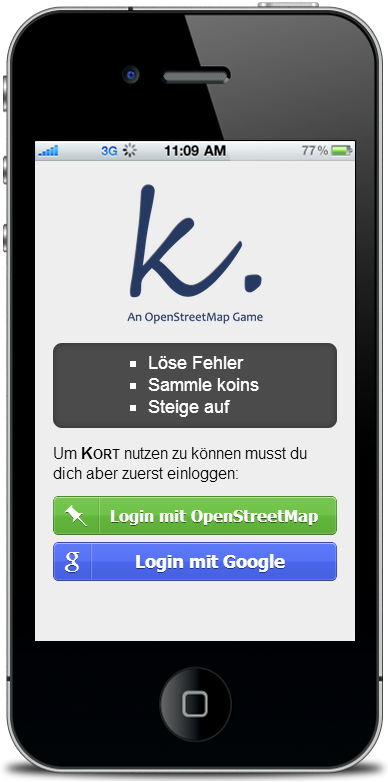
\includegraphics[width=0.3\textwidth]{images/screenshots/kort-screenshot-login}}
\hfill
\subfigure{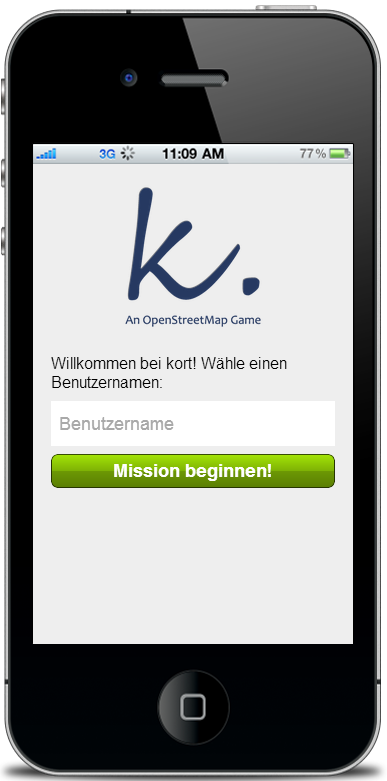
\includegraphics[width=0.3\textwidth]{images//screenshots/kort-screenshot-choose_username}}
\hfill
\subfigure{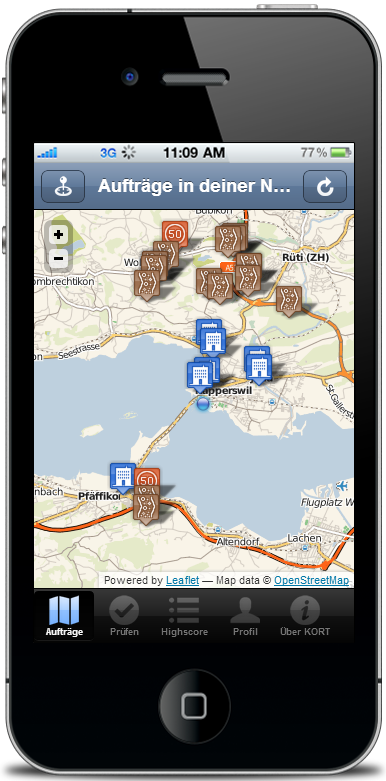
\includegraphics[width=0.3\textwidth]{images/screenshots/kort-screenshot-bugmap}}
\end{figure}
\end{center}

% Einführung
\section{Einführung}
\subsection{Idee}


% Ziel
\subsection{Ziel}


% Analyse
\section{Analyse}

% Subfigure counter zuruecksetzen
\setcounter{subfigure}{0}

\subsection{Paper-Prototype}
Vor der Implementation der Oberfläche wurde ein Paper-Prototype des GUI-Designs erstellt.
Der Prototype besteht aus vier verschiedenen Hauptmasken und einem Overlay für den Login.

\subsubsection{Overlay: Login}
Beim ersten Starten der \gls{WebApp} erhält man die Möglichkeit sich über verschiedene Dienste anzumelden.
Beim Klick auf den jeweiligen Anbieter wird man zu diesem Weitergeleitet und kann sich dort anmelden.

\begin{figure}[H]
\subfigure[Login - Anbieterauswahl]{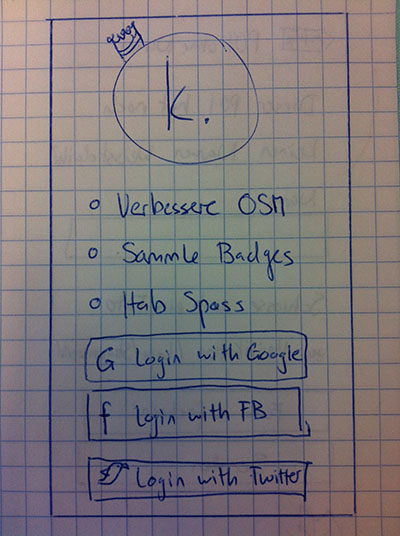
\includegraphics[width=0.43\textwidth]{images/paperprototype/kort-pp-startscreen}}
\hfill
\subfigure[Login - Loginformular des jeweiligen Anbieters]{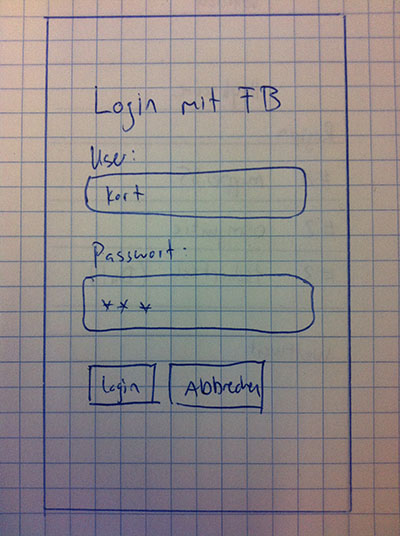
\includegraphics[width=0.43\textwidth]{images/paperprototype/kort-pp-login}}
\end{figure}

\subsubsection{Maske: Aufträge}
Ist der Login erfolgt erscheint die Maske mit den Aufträgen.
Darauf ist werden die bestehenden Fehler auf einer Karte angezeigt.
Es werden jeweils nur die Fehler angezeigt, welche sich in unmittelbarer Nähe vom eigenen Standort befinden.
Die Fehler werden mit einer Markierung auf der Karte dargestellt.

Durch Anklicken einer solchen Markierung öffnet sich die Detailansicht des Fehlers, worin sich der Fehler direkt beheben lässt.
Neben der Möglichkeit einen Lösungstext einzugeben, soll es auch möglich sein ein Beweis-Foto dazu hochzuladen.
Mit einem Klick auf Senden schliesst sich die Detailansicht und man sieht wieder die Karte.

\begin{figure}[H]
\subfigure[Aufträge - Karte mit Fehlern]{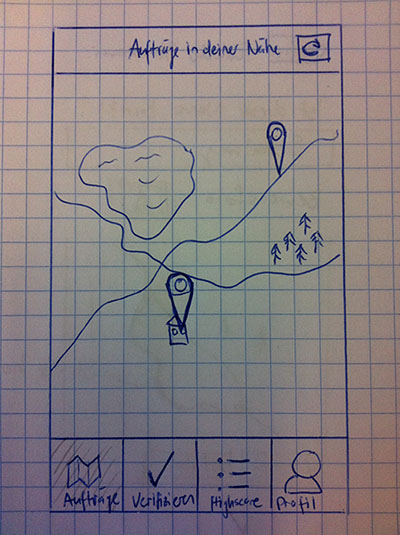
\includegraphics[width=0.43\textwidth]{images/paperprototype/kort-pp-bugs}}
\hfill
\subfigure[Aufträge - Detailansicht eines Fehlers]{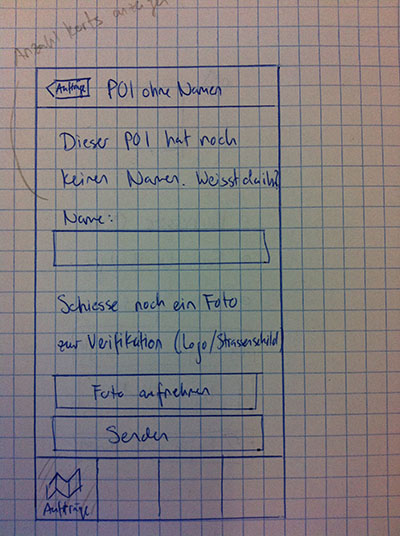
\includegraphics[width=0.43\textwidth]{images/paperprototype/kort-pp-fix}}
\end{figure}

\subsubsection{Maske: Verifizieren}
Auf der Verifikationsmaske werden die bereits gelösten Fehler in der Nähe angezeigt.
Sie sind gruppiert nach Anzahl nötigen Verifikationen, um sie zu OpenStreetMap zurückzusenden.

Per Klick auf einen Eintrag öffnet sich die Verifikationsmaske.
Darin wird der Fehlerlösungstext und das Beweis-Foto angezeigt.
Zusätzlich wird das betroffene OpenStreetMap-Objekt auf einer Karte angezeigt.
Man hat die Möglichkeit die Problemlösung als \emph{Korrekt} oder \emph{Falsch} zu werten.

\begin{figure}[H]
\subfigure[Verifizieren - Liste mit Fehlerlösungen]{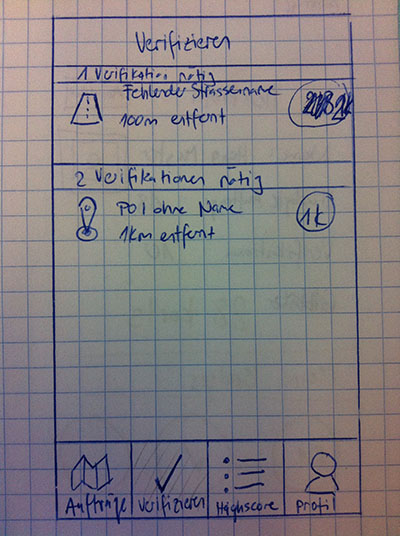
\includegraphics[width=0.43\textwidth]{images/paperprototype/kort-pp-verify}}
\hfill
\subfigure[Verifizieren - Detailansicht einer Fehlerlösung]{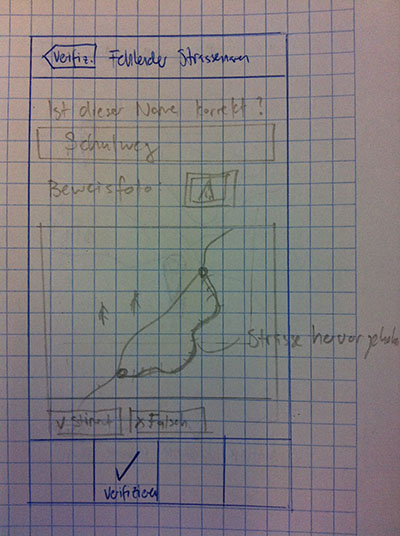
\includegraphics[width=0.43\textwidth]{images/paperprototype/kort-pp-verify_detail}}
\end{figure}

\subsubsection{Masken: Highscore / Profil}
In der Highscore-Maske hat man die Möglichkeit sich mit anderen Spielern vergleichen.
Man sieht seine eigene und die Platzierungen der anderen Spieler.
Es werden Highscores für verschiedene Kategorien (z.B. Regional, Weltweit) angezeigt.

Im Profil sieht man einen Steckbrief seines eigenen Benutzers.
Es wird angezeigt wieviele Aufträge man gelöst und wieviele Verifikationen man getätigt hat.
Zusätzlich werden die Gesamtanzahl der gesammelten Punkte und die gewonnenen Badges angezeigt.
Die Profil-Maske bietet zudem die Möglichkeit sich von der App abzumelden.

\begin{figure}[H]
\subfigure[Highscore]{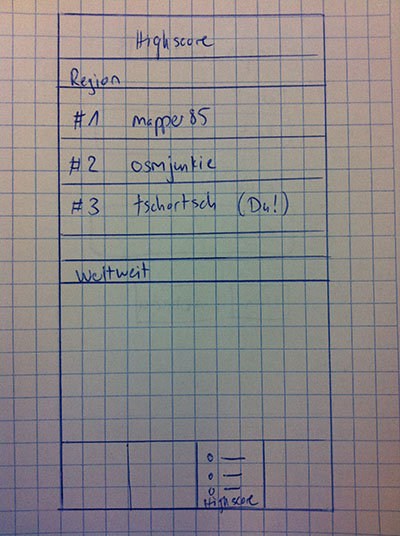
\includegraphics[width=0.43\textwidth]{images/paperprototype/kort-pp-highscore}}
\hfill
\subfigure[Profil]{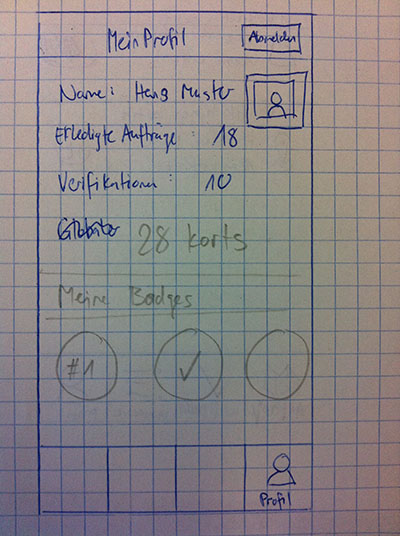
\includegraphics[width=0.43\textwidth]{images/paperprototype/kort-pp-profile}}
\end{figure}
